\begin{figure}
\centering
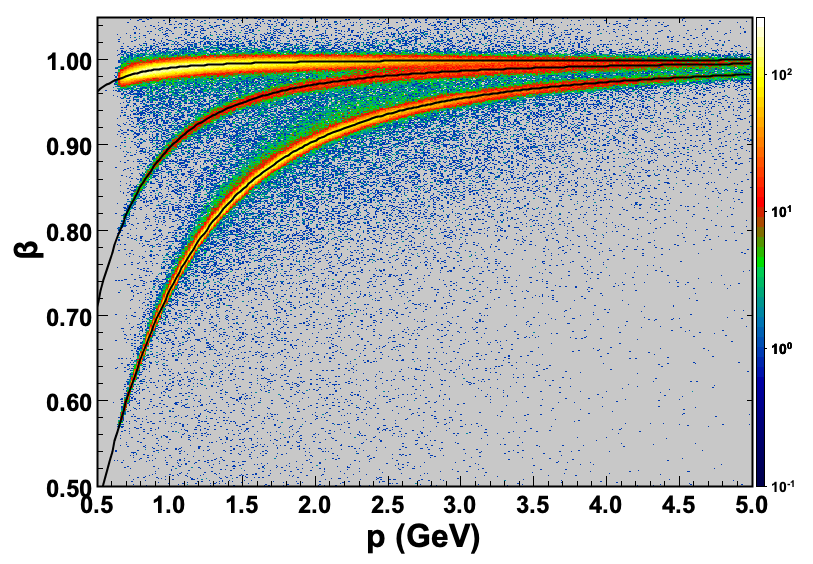
\includegraphics[width=0.45\textwidth]{pics/ftof_betap.png}
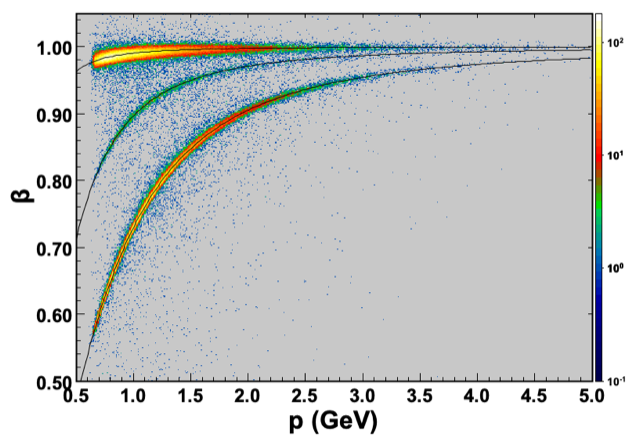
\includegraphics[width=0.45\textwidth]{pics/ft_betap.png}
\caption{Beta versus momentum for events with start time from an electron in the FD (top plot) and in the FT (bottom plot).}
\label{fig:betavsp}
\end{figure}

\subsection{Event Builder}\label{sec:eb}
The Event Builder is the last service in the reconstruction algorithms, and performs a series of functions:
\begin{itemize}
    \item collect information from upstream services
    \item correlates information from subdetectors into particles
    \item perform a general particle identification scheme
    \item organize the resulting information into a standardized, persisted data bank structure
\end{itemize}
The service is run twice with identical algorithms, once using hit-based tracks, and later with time-based tracks, where the results of the hit-based event builder are used to initialize time-based tracking.

\subsubsection{Forming Particles}
First, one charged particle is assigned to each reconstructed track.  Associated calorimeter, scintillator, and Cherenkov detector responses are then assigned to that particle based on geometric coincidence between the response and track, with matching criteria corresponding to the given detector.  The geometric matching is based on distance of closest approach between the track and response, where an example is shown in Figure \ref{fig:ebmatch}.

Then, a similar procedure is followed for creating neutrals particles, except seeding is with unassociated ECAL (for the forward detector) and CND (for the central detector) responses instead of tracks.

\begin{figure}
\centering
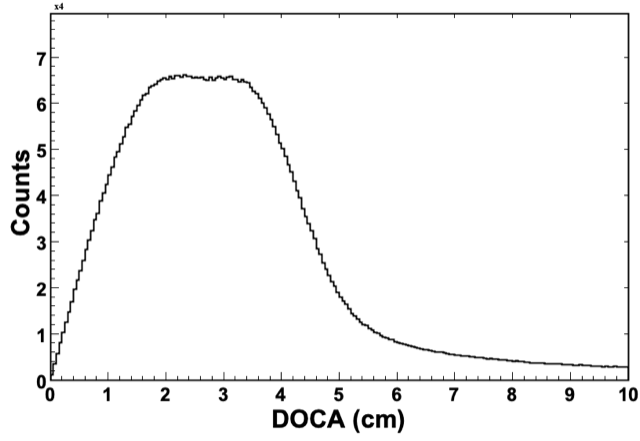
\includegraphics[width=0.45\textwidth,height=0.2\textheight]{pics/pcal-doca.png}
\caption{Example geometric matching criteria:  distance of closest approach between track and calorimeter clusters.\label{fig:ebmatch}}
\end{figure}

\subsubsection{Event Start Time}
A start time is assigned to the entire event, which serves as our most precise reference time on which all time-based particle identification relies.  This is based on the optimal charged particle candidate in the forward detector with an associated FTOF timing response, prioritized as
\begin{enumerate}
    \item $e^-$
    \item $e^+$
    \item positive track, assumed a $\pi^+$
    \item negative track, assumed a $\pi^-$
\end{enumerate}
where only the candidate with the highest momentum in each group is considered.

A parallel event start time is determined from the FT to facilitate physics analyses and triggers where the primary scattered electron is at very forward angles in the FT.  In this case, all combinations of charged particles in the FT and FD are considered.  The particle in the FT is assumed to be an electron, all hadron mass hypothesis are considered for the FD tracks, and the combination with the best time coincidence is chosen.  The timing of the resulting FT electron is then used to assign the start time.


\begin{figure}
\centering
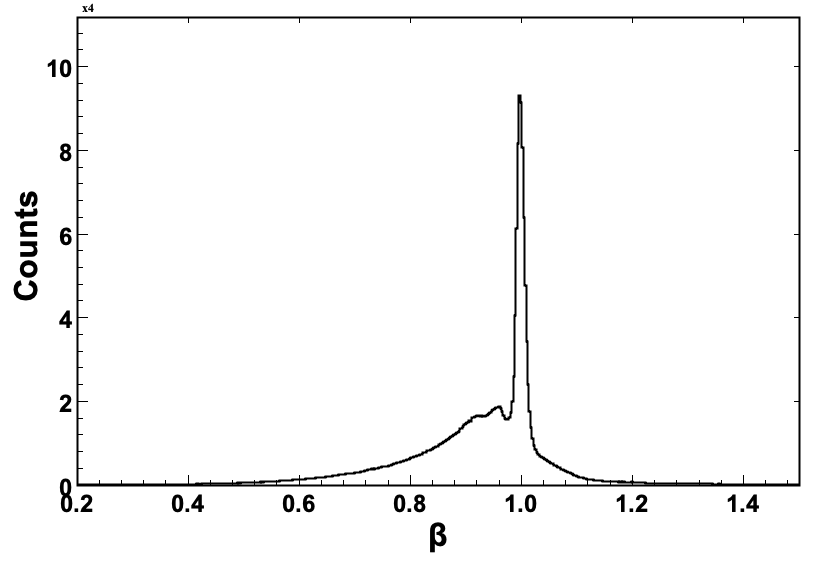
\includegraphics[width=0.45\textwidth]{pics/neutral_beta.png}
\caption{Beta for neutral particles as measured by the ECAL, showing a sharp peak at $\beta=1$ from photons and a broader, slower distribution from neutrons. TO BE REPLACED WITH NEW FIGURE AFTER FIX OF PCAL CLUSTER.}
\label{fig:neutbeta}
\end{figure}

A correction to the start time is then performed using the RF signal from the accelerator, combined with the event vertex position.  This effectively aligning the event start time to our best measure of bunch-crossing time at the primary interaction in the target.

The uncorrected, measured vertex time of a particle, $t_v$, can be written as
\begin{equation}
    t_v = t-\frac{l}{\beta c},
\end{equation}
where $t$ is the measured time response (e.g. in a scintillator), $l$ is the path length between the primary interaction vertex and that response, and $\beta$ is the speed of the particle.  We can then construct a correction to align it with the closest bunch crossing time:
\begin{eqnarray*}
\Delta t_{RF} &=& t_v + (z_0-z_v)/c - t_{RF} - N/2/f_{RF}, \\
\Delta t^{\prime}_{RF} &=& mod(\Delta t_{RF},1/f^{RF})-1/2/f_{RF},
\end{eqnarray*}
where $f_{RF}$ is the frequency of the accelerator, 250 MHz or 500 MHz, corresponding to 2 ns or 4 ns bunch spacings, $t_{RF}$ is the measured, calibrated RF time for the event, and $z_0$ is the target center and enters due to its use as a calibration reference.

The resulting, RF- and vertex-corrected start time for the event is then given as
\begin{equation}\label{eq:starttime}
t^{\prime}_v = t_v - \Delta t^{\prime}_{RF}.
\end{equation}

\begin{table}[htpb]
  \begin{center}
    \begin{tabular}{|c|cccccc|}\hline
          & \multicolumn{6}{c|}{Truth}\\        
          & $e$  & $\pi$ & $K$  & $p$  & $n$  & $\gamma$ \\\hline
  $e$     & 0.98 &       &      &      &      &          \\ 
  $\pi$   &      &  0.93 & 0.10 & 0.00 &      &          \\ 
  $K$     &      &  0.03 & 0.80 & 0.00 &      &          \\ 
  $p$     &      &  0.03 & 0.02 & 0.98 &      &          \\ 
  $n$     &      &       &      &      & 0.66 &   0.01   \\ 
 $\gamma$ &      &       &      &      & 0.14 &   0.95   \\\hline 
    \end{tabular}  
  \caption{Particle identification matrix for the FD acceptance, based on simulated hadrons and photons between 1 and 2.5 GeV momentum, and electrons up to 9 GeV.  The diagonal elements are correctly identified, while the off-diagonal elements are misidentified.  Detector inefficiencies are included.}
  \label{table:pidmatrix}
  \end{center}
\end{table}

\subsubsection{Particle Identification}
The next stage is a basic particle identification scheme.  This is intended to be loose to accommodate a variety of physics analyses, while persisting the necessary information to easily tighten the criteria later.

For charged particles, first calorimetry and Cerenkov information is used to positively identify $e^-/e^+$ candidates.  If the measured energy deposition is consistent with the expected sampling fraction of the ECAL, and the photoelectron response from the HTCC is consistent with $\beta\sim1$, the particle is assigned as an $e^-$ or $e^+$ depending on sign of the track's curvature.

Remaining charged particles are then assumed to be hadrons and assigned an identity based solely on timing information, where the $p/K/\pi$ candidate giving the smallest timing residual is assigned.  This is equivalent to the closest mass hypothesis curve in Figure \ref{fig:betavsp}.

For neutral particles, identity is assigned only for neutrons and photons, based only on timing and topological information.  If the particle timing results in $\beta\sim1$, then photon is assigned, otherwise neutron is assigned.  For the forward detectors this is based on ECAL, while for central it is based on CND.  For photons in the forward detector, momentum is then assigned based on the ECAL sampling fraction.  For neutrons, momentum is assigned based on the measured $\beta$ and neutron mass.

An identification quality factor, in the form of a signed-$\chi$, is assigned based on the relevant detector responses and their resolutions.  For $e^-/e^+$ the resolution-normalized distance from the expected ECAL sampling fraction is used, while for charged hadrons the resolution normalized time-difference is used.

\subsubsection{Persistence}
The resulting information is organized into standardized output bank structures for physics analysis, see \ref{sec:dsts}.  This includes particle four-vectors, all their associated detector responses, and global event information such as beam RF and helicity information.


\begin{figure}
\centering
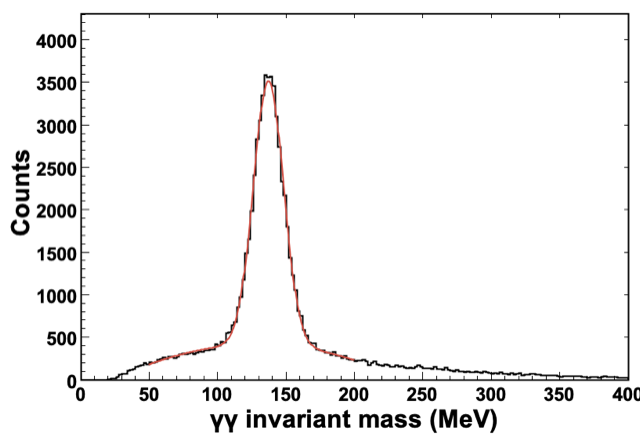
\includegraphics[width=0.45\textwidth]{pics/ecal_pi0.png}
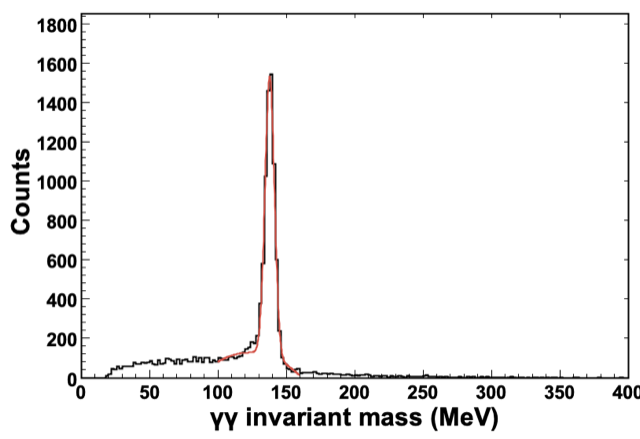
\includegraphics[width=0.45\textwidth]{pics/ft_pi0.png}
\caption{Reconstructed $\pi^{0}\rightarrow \gamma \gamma$ candidates using photons detected in the ECAL (top plot) and FT (bottom plot). The plots are based on simulations of Semi-Inclusive Deep Inelastic Scattering (SIDIS) events generated based on PYTHIA~\cite{clasdis}}
\label{fig:pi0mass}
\end{figure}
\subsubsection{Particle Identification Performance}
The accuracy of the particle identification algorithm that is currently implemented can be estimated from Monte Carlo simulations where the assigned PID can be compared to the true one. Table~\ref{table:pidmatrix} shows the particle identification matrix for the forward detector acceptance. The values are based on simulations of electron-hadron or electron-photon pairs with hadron and photon momentum in the range 1-2.5 GeV and electron momentum in the range 1-9 GeV. The diagonal elements corresponds to the cases where the particle is correctly identified and the off-diagonal ones to the cases were the particle is misidentified. It should be noted that the resulting values are strictly related to the PID algorithm currently in use and on the timing resolutions implemented in the Monte Carlo simulation. Increase of the diagonal element values and corresponding decrease of the misidentification probability is expected as for example information from the CLAS12 Cerenkov detectors and the CLAS12 RICH in particular will be integrated in the algorithm.

Another measure of the particle identification performance for neutrals is given by the reconstruction of $\pi^0$ decaying to two photons. Fig.~\ref{fig:pi0mass} shows the $\gamma \gamma$ invariant mass reconstructed from the Forward Electromagnetic Calorimeter and from the Forward Tagger.


